\documentclass[11pt]{article}

%packages
\usepackage{geometry}
\usepackage[english]{babel}
\usepackage{amsmath}
\usepackage{graphicx}
\usepackage[colorlinks=true, allcolors=black]{hyperref}
\usepackage[detect-all]{siunitx}
\usepackage{caption}
\usepackage{subcaption}
\usepackage[natbibapa]{apacite}

\newgeometry{
    top=2cm,
    bottom=2cm,
    left=3cm,
    right=3cm
}

% title page
\begin{document}
\begin{titlepage}
	\centering
	%emblem of Uni Osnabrueck
	{\scshape\LARGE University of Osnabrueck \par}
	\vspace{1cm}
	
\includegraphics[width=0.5\textwidth]{images/Logo-Uni-Osnabrueck.jpg}\par\vspace{2cm}
	\vspace{0.75cm}
	{\scshape\Large Implementing ANNs with TensorFlow\par}
	\vspace{1.5cm}
	{\huge\bfseries Turtle Recognition Using Deep Convolutional Neural Networks\par}
	\vspace{1.5cm}
	{\Large\itshape Dennis Hesenkamp, Lennart Zastrow,  Madhuri Ramesh\par}
	\vspace{1.5cm}
	supervised by\par
	\textsc{Charlotte Lange}
	\vfill

	{\large \today\par}
\end{titlepage}

\tableofcontents
\newpage

\begin{abstract}
    Here is room for an abstract.
\end{abstract}

\section{Background}

Three-fifths of all turtle species worldwide are on the verge of extinction or are already severely threatened. According to a U.S. study published in the journal BioScience, this makes turtles the most endangered vertebrates in the world, ahead of mammals, birds, fish, and amphibians.

Sea turtles are known as indicator species which means that their presence and abundance reflect the health of the wider ecosystem. Therefore, increasing our ability to identify and understand them can enhance our ecological understanding.

Not only for their own sake, but they also contribute significantly to a healthy ecosystem. The herbivores, carnivores, or omnivores are at the same time hunters, pest controllers, and food sources for other animals. The scavenging species, for example, ensure a clean environment, and the herbivorous turtles make an important contribution to spreading plant seeds.

For many sea turtles, sea grass is the main food source. Sea grass grows in thick beds on shallow seabeds. Constant feeding by sea turtles on this grass keeps the beds in order and prevents them from becoming long and unhealthy. Because these sea grass beds are prime locations for small fish to breed and spawn, healthy sea grass beds are critical to populations of small fish living in the oceans. Without this contribution from sea turtles, the ocean ecosystem would be out of balance.

While sea turtles spend most of their lives in the ocean, they come to the beach to lay their eggs. This important part of a turtle's life also has an important impact on a beach's ecosystem. Without plants like beach grasses, the beach would succumb to erosion. These plants are fertilized by eggs that do not hatch and by turtle droppings on the beach. This nutrition is essential for the survival of the beach ecosystem.

Humans are making it difficult for the turtles to survive. The animals are suffering from climate change, habitat destruction, excessive trade in live animals, the sale of their meat and shells, and environmental pollution.
For example, Australian scientists estimated that one in five sea turtles now dies from eating too much plastic. With 14 swallowed plastic particles, the risk of death increases to 50 percent. At 200 pieces swallowed, the sea turtle is no longer viable. The plastic pieces get stuck or cause internal injuries.

The greatest threat to turtles, however, is and remains humans. In some regions of the world, turtles are considered a delicacy; worldwide, they are kept as exotic pets. The meat of larger species ends up on markets in Asia, Africa, and Latin America, for example, while smaller species are traded internationally primarily as pets. The turtle shell ends up in the powdered form in pills and pastes used in traditional Asian medicine (including TCM). Some species, which are said to have a special medicinal effect, such as the three-striped hinge back turtle (Cuora trifasciata) achieve prices of several thousand US dollars per animal. Even in Europe, turtles can still be ingredients in TCM formulations.
\section{Grant Species Preservation Through Population Census}


The ability to distinguish between individuals of the same species is a fundamental tool for modern animal welfare. To ensure the protection of individuals, it is crucial to identify their whereabouts and movement patterns. Because sea turtles are a powerful indicator of overall ecosystem health, accurate identification serves to enhance our ecological understanding. Implicitly, this means that ensuring species conservation can be generated and optimized.  


\subsection{Turtle Tagging}
In the past, the detection and tracking of individuals was done by attaching tags to the fins of the individuals found. This method is severely compromised by the loss of tags and thus the successful tracking of population dynamics is not guaranteed. Basically, the use of \emph{flipper tags} was common, which are mostly made of metal and plastic. This method is very costly due to the extraordinarily long life span of the turtles, which means that the flipper tags were lost or identification was no longer possible due to wear and tear of the material.


\subsection{Photographic Identification}
Just as the human finger print, turtles have unique and time-stable facial scales by which they can be identified \cite{Carpentier2016}. Photographic identification has become the method of choice over time as it is non-invasive and low-cost. Due to the advances in machine learning and object identification, we are able to identify turtle individuals with algorithms as opposed to humans manually searching through a database of images. The goal of such machine learning algorithms is to assign a unique ID to each individual if it already exists in the database and to create a new ID if a new individual has been sighted.
\section{Convolutional Neural Networks}


In the field of machine learning, especially in the deep learning sector, a convolutional neural network (CNN) is a deep learning algorithm. It can take an input image and reproduce an identification of the object with a certain probability. The special feature of a CNN is that it is able to learn filters of different types (e.g. horizontal lines, vertical lines, etc.). A convolutional neural network has a characteristic structure in terms of its layers. It is structured in convolutional, pooling, and fully connected layers. The arrangement of alternating convolutional and pooling layers allows a more accurate and complex analysis of the image. The first layers focus on shapes and colors, while later layers contribute to the identification of more complex details for the recognition of the overall image.

CNNs have been around for a long time already: LeCun (1989), Fukushima's \emph{neocognitron} (1979) \textbf{NEED CITATION}


\subsection{Convolutional Layer}
The convolutional layer is the key component of a CNN. It contains a certain set of filters, also called kernels. The parameters of the filter are learned over the course of the training. The filter interacts with the image and convolves it. From this convolution, an activation map is created which is calculated from the dot product between each element of the filter and the input. The weights in the filter are maintained as the filter moves across the image. However, these weights adjust during backpropagation and the associated gradient descent to achieve the most accurate results. 

%picture of Convolution 
\begin{figure}[htb]
    \centering
    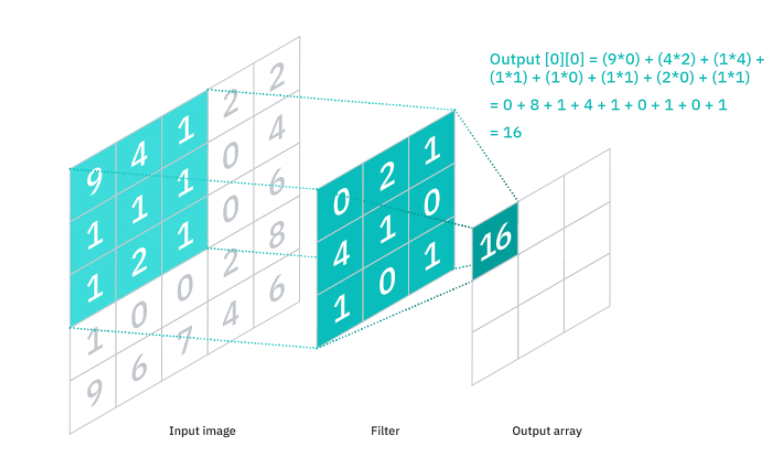
\includegraphics[width=7cm]{images/conv_layer.jpg}
    \caption{Convolutional Layer}
    \label{fig:convLayer}
\end{figure}


\subsection{Pooling Layer}
Since a great increase in dimension occurs through the use of a convolutional layer, a dimension reduction is required in the next step to reduce the number of parameters of a CNN. This is achieved by the pooling layer. It has the advantage that the computational cost decreases drastically. Also, unnecessary details are omitted, which is helpful for the later image identification.The most commonly used pooling methods are maximum and average pooling. In figure \ref{fig:poolingLayer} you can see how a maximum pooling is performed, leading to a dimension reduction.

%picture of Convolution 
\begin{figure}[htb]
    \centering
    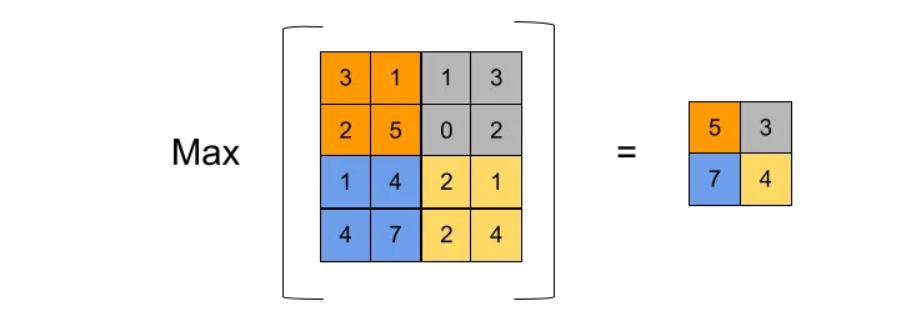
\includegraphics[width=7cm]{images/maxpooling.jpg}
    \caption{Max Pooling Layer}
    \label{fig:poolingLayer}
\end{figure}


\subsection{Fully-Connected Layer}
Since the individual pixel values of the input image are not directly connected to the output layer, a fully-connected layer is required which is directly connected to the output layer. The layer does the classification using the collected features from the previous layers. At the end, a softmax function is applied, which outputs a classification using probabilities between 0 and 1.

%picture of Convolution 
\begin{figure}[htb]
    \centering
    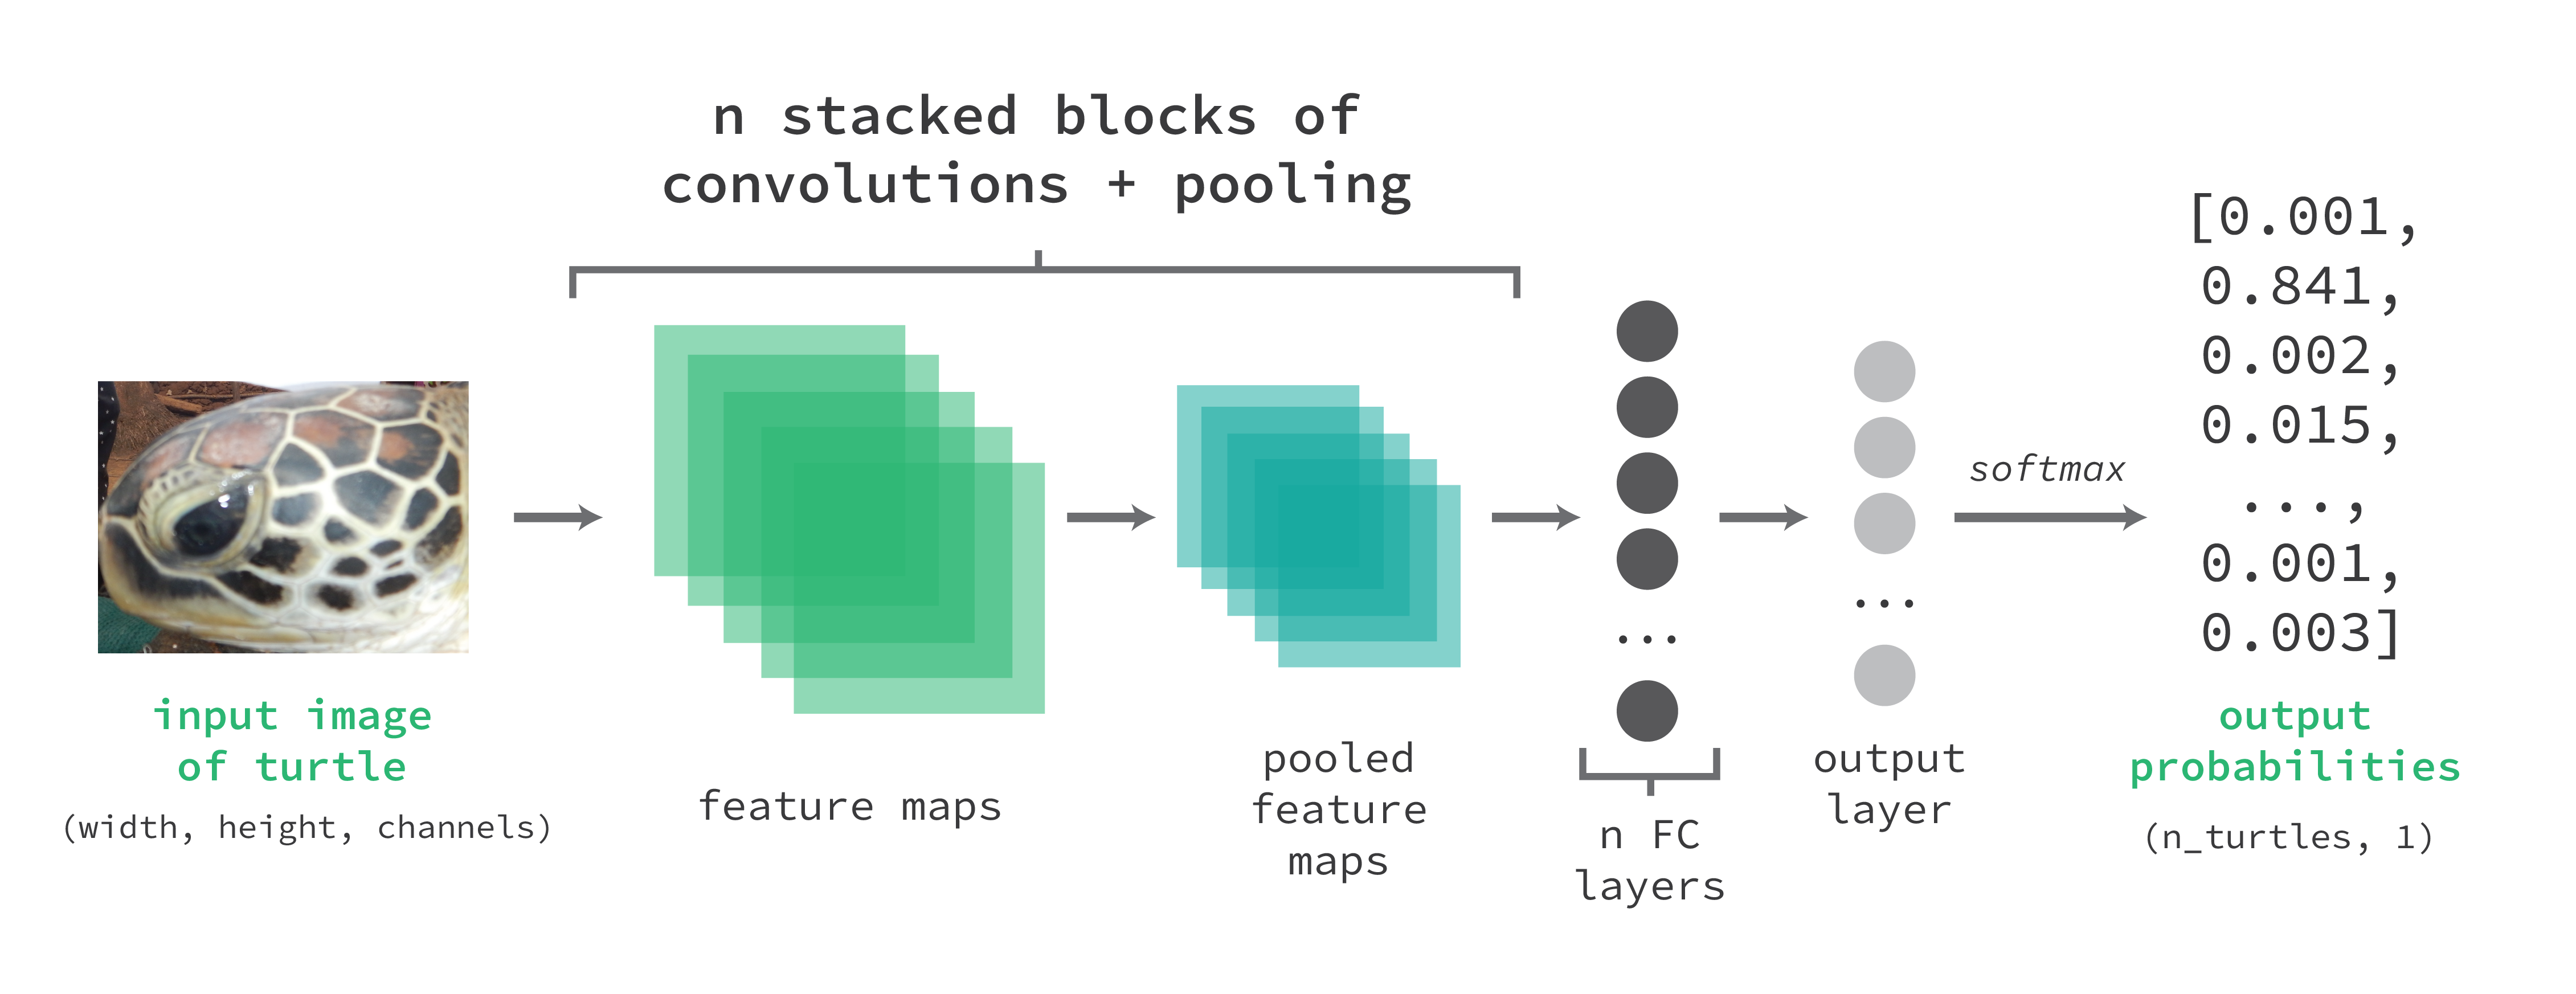
\includegraphics[width=10cm]{images/cnn_turtle_pooling.png}
    \caption{Turtle Image using CNN}
    \label{fig:turtleCNN}
\end{figure}
\section{Data}
The dataset is provided with the \emph{Turtle Recall: Conservation Challenge}\footnote{\url{https://zindi.africa/competitions/turtle-recall-conservation-challenge/data}} and consists of images of turtle faces. The images are labelled, each turtle has a unique ID. Besides the angle from which the image was shot (top, right, left) and the ID, no further info is provided about the images.

The images themselves have three colour channels, come in different sizes, and many have timestamps or handwritten identification tags in the background. They are split in three parts: a set of images for training, one for testing, and a large set of extra images.

The training set consists of 2145 images from 100 unique turtles. The set with the extra images comes with an additional almost 11000 images from 2231 different turtles, some already contained in the train set. This yields a total of about 13000 images and 2265 turtles. The test set only comes with images but without the annotation of turtle IDs, as it is meant to be used for model evaluation in the priced competition. However, this means that the test images are without use for our purpose.

Because the training set is rather small, we also make use of the extra images. A quick exploratory analysis shows that the dataset is both hugely unbalanced and that there are only less than 6 images per turtle on average, with a median number of 3 images per turtle. Because such a small amount of data per class will likely lead to very poor approximation results, we decide not to use the entire available data.


\subsection{Preprocessing}
Before actually using the images and feeding them into a neural net, we need to perform some necessary as well as some optional preprocessing steps in order to bring the image data into a more helpful format.

As a first step, we get rid of any turtles with less than a specified number of images in the dataset. We require each turtle to be represented by at least 10 images in the dataset. This reduces the total number of turtles to 253 and the total number of images to roughly 5000. Turtles now have an average of 20 images and a median of 14 images. There is still a considerable imbalance in the data, as can be seen in figure \ref{fig:images_per_turtle}.

\begin{figure}[h]
    \centering
    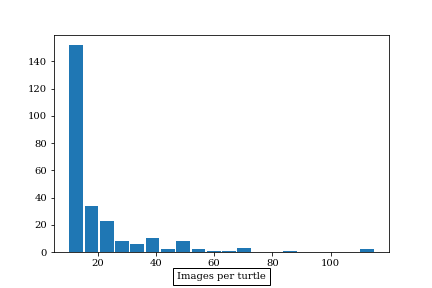
\includegraphics[width=12cm]{images/images_per_turtle.png}
    \caption[Number of images per turtle]{Number of images per turtle. The left skew of the distribution means there are many images with the minimum amount of images, while only a few have considerably more.}
    \label{fig:images_per_turtle}
\end{figure}

We further crop and resize the images such that they are all in the same shape and size, namely $224\times224$ pixels. Before doing any computations on the image data, we also convert them to numerical arrays, yielding us a three-dimensional array of size $224\times224\times3$ for each used image. Since the colours are in the RGB colour space, the values are now in the range \numrange{0}{255}, which we normalise to a range of \numrange{0}{1}. This has been shown to increase training speed of deep networks \citep{Ioffe2015}. We further apply a one-hot encoding to the classes, as the alpha-numerical strings the turtle IDs are supplied in are rather meaningless to a neural net. At this point, we are technically ready to feed the images into a network for training.


\subsection{Data Augmentation}
The dataset, unfortunately, contains very little data unevenly distributed among the classes. A low number of training examples per class can lead to the class not being learned efficiently and may even impede the entire training process \citep{Huh2016}. To avoid this, we apply a set of basic augmentation techniques to multiply the data available for training:

\begin{description}
    \item[Image rotation] We rotate the images by 90, 180, and 270 degrees. This immediately quadruples the available data. The basic characteristics of the pattern on the head of the turtle are preserved.
    \item[Gaussian filter] We also apply a Gaussian filter to introduce a blur and reduce detail in the image. Mathematically, this is the same as convolving the images with a Gaussian function.
    \item[Random HSV] The HSV colour space uses hue, saturation, and value to describe colours, whereas the RGB colour model uses a linear combination of the colours red, green, and blue to describe the same. We transform the RGB values to HSV, randomly modify them within a specified range, and convert back to RGB.
    \item[Additive noise] Lastly, we add random numerical values, sampled from a normal distribution with very low standard deviation, to the existing image values, followed by clipping the values within range \numrange{0}{1} (our normalisation range).
\end{description}

Applying the above techniques, we have enhanced our dataset and also somewhat shifted the distribution of images per turtle to be more desirable. Further common augmentation techniques include random brightness shifts, grey level mapping, histogram equalisation, image shifting and shearing. Example images of the used augmentations can be seen in appendix \ref{apx:augmentedImages}.
\section{Models}

\subsection{AlexNet}
\citeauthor{Krizhevsky2012} have presented their influential \emph{AlexNet} in \citeyear{Krizhevsky2012}. It consists of only five convolutional layers, some additional max-pooling layers and three fully connected layers at the end, so its structure is rather simple. Nonetheless, it is packed with more than 40.000.000 trainable parameters (the fully connected layers at the end are very large), making it not exactly computationally cheap to train. An AlexNet was supposed to serve as our baseline model from which we wanted to build things up.

\subsection{EfficientNet}
We then implemented a pre-trained EfficientNet with custom top layer. The EfficientNet model family was first introduced in 2019 (\citeauthor{Tan2019}) with the idea of providing scalable CNN architectures. Multiple networks of different size for image classification purposes were introduced, many achieving better results than state-of-the-art models like MobileNet and ResNet while being significantly smaller in terms of depth, width, and image resolution \citep{Tan2019}. Two years later, a second, even more powerful and efficient generation was introduced: EfficientNetV2 \citep{Tan2021}. For our purposes, given the low input resolution of $224\times224$, the model of choice is the EfficientNetV2-B0 -- the smallest model of the ensemble. The model is pre-trained on ImageNet21k and we implemented a custom fully-connected layer at the end to match our classification task.

\subsection{InceptionNet}
For an additional comparison, we implemented yet another supposedly very efficiently designed CNN, the InceptionV3 as introduced by \citeauthor{Szegedy2015} in \citeyear{Szegedy2015}. Its computational low cost makes the Inception architecture an attractive choice when resources are limited, e.g. in mobile scenarios. The inception network was a milestone in the development of CNN classifiers. It achieved extremely high accuracies on the ImageNet dataset for example the inception v3 network achieved an accuracy of 78,1 percent. 
The fundamental idea behind the inception network is the inception block. In a traditional convolutional neural network layer, the previous layer's output is the input of the next layer until the state of prediction is accomplished. The inception block takes apart the individual layers. The previous layer's output is passed to four different operations in parallel and concatenates the outputs from all these different layers. So instead of constructing a deeper network, a “ wider network” is provided. The naive approach consists of a 1x1 convolution layer, a 3x3 convolution layer and a 5x5 convolutions layer followed by a max-pooling layer and a concatenation layer. Due to the high computational cost especially with the 5x5 filter, the 1x1 is first added to the naive inception module. This leads to a computational reduction of 90 percent.
Additionally, the 1x1 convolutional filters allow learning cross channel patterns across the depth of the input data. 


%picture of Convolution 
\begin{figure}[htb]
    \centering
    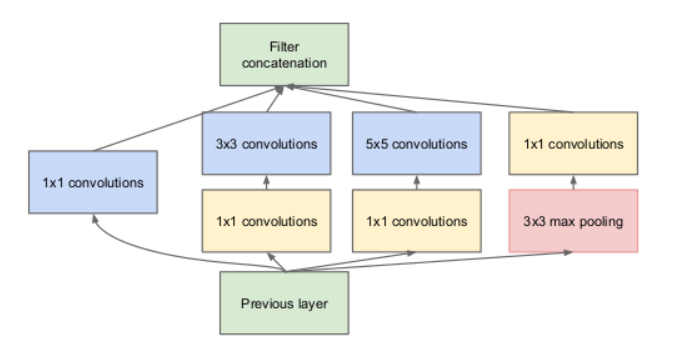
\includegraphics[width=7cm]{images/InceptionNet.jpg}
    \caption{Inception Block}
    \label{fig:incepblock}
\end{figure}


- balance of depth and width within network
- aggressive regularisation
- inception architecture already introduced by GoogLeNet (2014)


\subsection{Hyperparameters}
For simplicity, we use more or less the same hyperparameters for all networks.

Categorical cross-entropy: Cross-entropy loss is differentiable with respect to the logits and thus can be used for gradient training of deep models.
\section{Evaluation}


When finally wanting to run and evaluate the models, we encountered problems with the execution of our pipeline. It turned out that the training process requires dramatically more computational resources than we anticipated - more, at least, than our local machines could handle. We tried different approaches to cope with this problem: As a first step, we skipped the AlexNet as baseline model. It has a huge number of trainable parameters compared to the pre-trained EfficientNetV2 (small amount of trainable parameters) and InceptionV3 (somewhat in the middle between the former two), requiring much more backpropagation computations within the training. Unfortunately, just having fewer trainable parameters did not reduce the computational load enough for us to be able to train the models.

\textbf{INSERT TABLE WITH PARAMS}

The next logical consequence for us was to reduce the size of the dataset. We initially augmented the data, increasing the size of the dataset roughly 10-fold, to enable the models to better learn features of the turtle head patterns and avoid overfitting. Step by step, we cut out the different augmentations until we were back to the original, non-augmented dataset. Even this dramatic decrease of dataset size back to around 5000 images did still not allow us to train the models properly. We then went on to experiment with different buffer sizes for the shuffle procedures and different batch sizes to reduce the load on the RAM. Although decreasing both of these parameters seemed to free up RAM, a full training was still not possible. The EfficientNetV2, which was for now the model on which we tried to train, was able to run the fitting for 1-3 epochs before sessions crashed due to full RAM. Even further reducing the dataset size by increasing the number of minimum images per turtle from 10 up to 15, which lead to a further reduction of the total number of images to little over 3000, did still not allow for successful training.

CNNs can generally be scaled along three dimensions: changing the depth of the network, i.e. the number of layers, the width of the network, e.g. by increasing the number of channels per convolutional layer, or by changing the resolution of the input images. Because we did not want to make major changes to the layer architecture of the models we use, we decided that downsampling the images would be the next measure to explore. The resolution we used so far yields $224\times224\times3=150528$ values per image, we reduced to $160\times160$ pixels with a resulting decrease of $\raisebox{-0.9ex}{\~{}} 50\%$ with regard to image values: $160\times160\times3=76.800$. Reducing the dataset size (although not the number of samples) again by half with this approach, we managed to successfully train the EfficientNetV2. We were not happy with this approach since reducing the image size potentially gives rise to unrecoverable loss of important information \citep{Zhang2011}. Further, both the EfficientNetV2 and the InceptionV3 expect input sizes of $224\times224$.

Because of this, we turned to Google Colab to execute our pipeline. The resources there allowed us to return to the previous resolution of $224\times224$ pixels. Treating the minimum number of images per turtle (which directly affects the number of samples in the dataset) as a first hyperparameter to explore - we still could not run the training with the entire augmentation pipeline due to RAM restrictions - we found a dataset size of approximately 5000 images to max out on Colab's freely available resources. A table with how the minimum number of images affects the dataset size and median number of images per turtle can be found in table \ref{tab:minImages} in appendix \ref{apx:minImages}. Further naïvely exploring the batch size, we found batches of 64 samples to best work with the computational resources while still allowing for a feasible training speed. The convergence behaviour did not seem to be significantly affected by different batch sizes.

A first run with both the EfficientNetV2 and InceptionV3 for 10 epochs to establish a baseline yielded the results shown in figure \ref{fig:efficientInceptionComparison}.

\begin{figure}[h!]
    \centering
    \includesvg[width=8cm]{images/efficient_inception_comparison.svg}
    \caption{Categorical accuracy on training and validation data for EfficientNetV2 (train: orange, validation: blue) and InceptionV3 (train: light blue, validation: pink).}
    \label{fig:efficientInceptionComparison}
\end{figure}

The EfficientNetV2 is able to achieve accuracy $97.02\%$ on the training set while the InceptionV3 - pre-trained on the same ImageNet21K - achieves $90.18\%$. Validation accuracies are $49.83\%$ and $17.01\%$, respectively, and test accuracies are $50.42\%$ and $16.25\%$, suggesting that the InceptionV3 actually overfits on the training data. Although no definite convergence behaviour could be seen at this point, we decided to focus on the EfficientNetV2 -- mainly due to the limited computational resources. We can, however, not draw any meaningful conclusion regarding the InceptionV3 since we did not explore this direction any further.

After establishing this baseline using only non-augmented images, we went on to assess to what extent the different augmentations influence model performance. We first reduced the size of the dataset by increasing the minimum number of images per turtle to 13 (from 10), and then augmented a part of this data using only a single augmentation technique to get the image number up to roughly 5000 again. The comparison between baseline and augmentations, which can be seen in figure \ref{tab:augmentationComparison}, has to seen skeptically, though, because increasing the number of required images per turtle does a) significantly reduce the number of classes (unique turtles) from 254 to 150 and b) provide more total data per class, which theoretically should allow the model to better capture the underlying distribution.

\begin{table}[h]
    \centering
    \begin{tabular}{l|l|l|l|}
    \cline{2-4}
                                        & \textbf{Train} & \textbf{Validation} & \textbf{Test} \\ \hline
    \multicolumn{1}{|l|}{Baseline}      & 97.02\%        & 49.83\%             & 50.42\%       \\ \hline
    \multicolumn{1}{|l|}{180° rotation} & 93.14\%        & 89.38\%             & 58.98\%       \\ \hline
    \multicolumn{1}{|l|}{Gauss-filter}  & 96.76\%        & 96.72\%             & 63.80\%       \\ \hline
    \multicolumn{1}{|l|}{Random HSV}    & 98.67\%        & 98.46\%             & 56.77\%       \\ \hline
    \multicolumn{1}{|l|}{Noise}         & 92.27\%        & 86.15\%             & 56.77\%       \\ \hline
    \end{tabular}
    \caption[]{Categorical accuracy of EfficientNetV2 on differently augmented datasets after 10 epochs.}
    \label{tab:augmentationComparison}
\end{table}

As can be seen, validation and test accuracies greatly benefit from all augmentations, with the Gaussian filtering considerably outperforming the other techniques on the test data.
\section{Open Questions}

We consider achieving a test accuracy of $63.80\%$ given the size and characteristics of the dataset after 10 epochs of training already a great success, but we could not evaluate the models for their full potential within the scope of this project. With more computational resources available, the next obvious step would be to increase the size of the dataset to include all augmentations while also including more turtles again by lowering the number of minimum images per turtle. Then, it would also be interesting to conduct a more thorough hyperparameter search, which was not feasible for us. For example, we only used Adam with standard parameters as optimizer because it is computationally efficient and requires little memory \citep{Kingma2014}. The EfficientNet model family has been trained with Hinton's unpublished RMSProp \citep{Tan2019}. Further, we only reported categorical accuracy as model evaluation metric. In the original Zindi competition, mean average precision at top 5 (MAP@5) has been suggested for this problem, probably because of the many classes to consider. Another interesting approach could be a less aggressive downsampling of the images. As proposed in the original competition, we scaled the images down to a resolution of $224\times224$, exactly the resolution that is also suggested as input for the EfficientNetV2-B0. As already discussed earlier, EfficientNet is a model family and B0 the smallest one in the ensemble. By scaling up the image resolution, it would not only be possible to include more information in the images themselves, but also to employ a larger and stronger model.

Further, we manually designed the augmentation. Doing so effectively is usually dataset-specific and requires expert knowledge in the image domain, as different techniques work best for different domains. \citeauthor{Cubuk2018} have proposed their AutoAugment image augmentation procedure in \citeyear{Cubuk2018}, in which a search space of augmentations is automatically explored to find the best procedures given the data at hand.

The competition on Zindi is not yet over at the time of writing this documentation, but the top-5 leaderboard scores already achieve a MAP@5 of more than $98\%$. We are excited to see which procedure ultimately works best on this problem.

\bibliographystyle{apacite}
\bibliography{references}

\newpage
\appendix
\Huge{\textbf{Appendices}}

\section{Augmented Images}\label{apx:augmentedImages}

\begin{figure}[h]
    \centering
    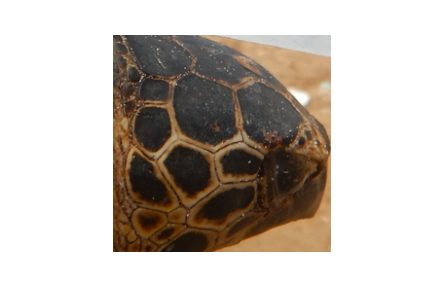
\includegraphics{images/turtles/base.png}
    \caption{Non-augmented image.}
    \label{fig:turtleBase}
\end{figure}

\begin{figure}[h!]
    \centering
    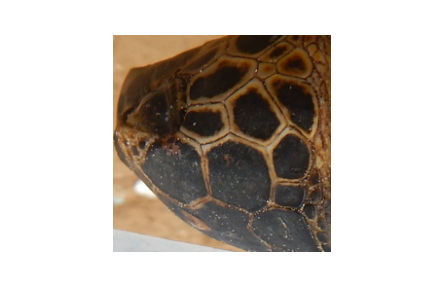
\includegraphics{images/turtles/rotated.png}
    \caption{Image rotated by 180 degrees.}
    \label{fig:turtleRotated}
\end{figure}

\begin{figure}[h!]
    \centering
    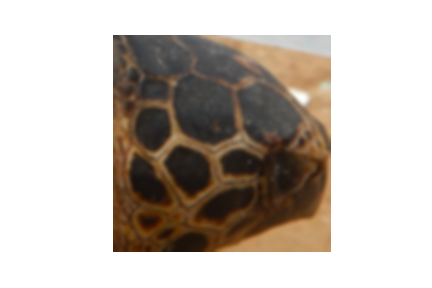
\includegraphics{images/turtles/gaussian.png}
    \caption{Image with Gauss-filter applied.}
    \label{fig:turtleGauss}
\end{figure}

\begin{figure}[h]
    \centering
    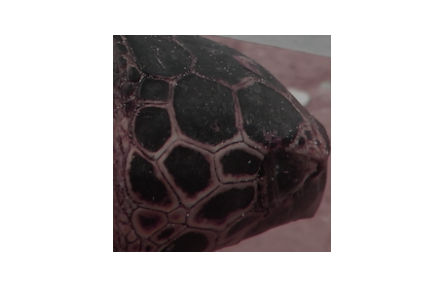
\includegraphics{images/turtles/hsv.png}
    \caption{Image with randomly changed HSV values.}
    \label{fig:turtleHSV}
\end{figure}

\begin{figure}[h]
    \centering
    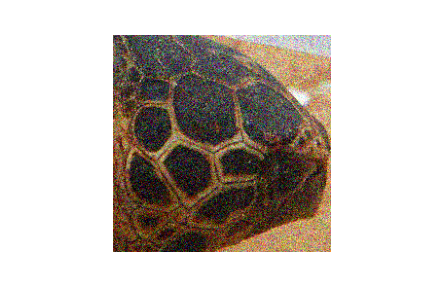
\includegraphics{images/turtles/noise.png}
    \caption{Image with added noise.}
    \label{fig:turtleNoise}
\end{figure}

\clearpage

\section{Dataset}\label{apx:minImages}
\begin{table}[h]
    \begin{tabular}{|l|c|c|c|c|c|c|c|c|}
    \hline
    \textbf{Min number images}                 & 8    & 9    & 10   & 11   & 12   & 13   & 14   & 15   \\ \hline
    \textbf{Images in dataset}               & 5846 & 5638 & 4990 & 4690 & 4338 & 3846 & 3560 & 3392 \\ \hline
    \textbf{Images per turtle (median)} & 12   & 12   & 14   & 15   & 16   & 18   & 21   & 22   \\ \hline
    \end{tabular}
    \caption[]{Dataset size in relation to number of images per turtle.}
    \label{tab:minImages}
\end{table}

\end{document}